\documentclass[runningheads]{llncs}

\usepackage[T1]{fontenc}
\usepackage[utf8]{inputenc}
\usepackage[english]{babel}
\usepackage{graphicx}
\usepackage{amsmath, amssymb}
\usepackage{booktabs}
\usepackage{subcaption}

\begin{document}

\title{Data Drift in a Seq2Seq Model for SSL Robot Trajectory Prediction}

\author{Ivan Yamasaki\inst{1}\orcidID{} \and
Marcos R. O. A. M\'aximo\inst{2}\orcidID{0000-0003-2944-4476} \and
Paulo Tasinaffo\inst{3}\orcidID{}}
%
\authorrunning{Ivan Yamasaki}
%
\institute{Aeronautics Institute of Technology, S\~ao Jos\'e dos Campos, Brazil}
%
\maketitle

\begin{abstract}
We investigate \textit{data drift} in a \textit{sequence-to-sequence} (seq2seq) model for robot trajectory prediction in the RoboCup Small Size League (SSL), where the model was trained on 2019 match data and evaluated across subsequent seasons under two prediction horizons. The contribution of this work is a systematic empirical assessment of the temporal robustness of the seq2seq predictor: we measure how performance---summarized by the \textit{Average Displacement Error} (ADE)---degrades over time and how this degradation compares with a Kalman-filter benchmark, providing the first longitudinal analysis of distribution shift for this class of neural trajectory predictors in SSL. Results show that the seq2seq ADE increases in years following training, characterizing drift-induced performance loss, while the relative advantage of the seq2seq over the Kalman grows, indicating that both methods are affected by the temporal shift but the Kalman filter loses predictive accuracy more steeply, as its fixed kinematic assumptions become increasingly misaligned with the evolving game dynamics. As complementary evidence, \textit{Ordinary Least Squares} (OLS) regressions relating ADE variation to Kolmogorov--Smirnov and Wasserstein drift metrics confirm that the error increase tracks measurable changes in the kinematic distributions of the matches.
\keywords{data drift \and Kalman filter \and RoboCup SSL \and seq2seq \and trajectory prediction}
\end{abstract}

\section{Introduction}

Trajectory prediction is a central task in autonomous systems subject to fast dynamics. In the RoboCup Small Size League (SSL)~\cite{kitano1997}, forecasting the future motion of robots supports planning, positioning, and real-time decision making. Sequence-to-sequence (seq2seq) architectures~\cite{sutskever} have proved effective for this kind of temporal forecasting; in the SSL context, Steuernagel and M\'aximo~\cite{seq2seq} showed that an encoder-decoder model with additive attention significantly outperforms the classical Kalman filter predictor in trajectory forecasting accuracy.

The SSL, however, is not a static environment. Over successive seasons, robot hardware has improved, rules have been updated, and team strategies have grown increasingly complex and coordinated. Faster robots, more agile maneuvers, and more sophisticated multi-robot tactics imply that the statistical patterns of robot motion present in one season are not necessarily representative of later years. This natural evolution of the competition motivates the study of \textit{data drift}: the performance degradation that occurs when a model trained on one data distribution is evaluated on samples from a shifted distribution in subsequent seasons. Data drift is a well-studied phenomenon in machine learning~\cite{gama2014}, yet its implications for trajectory predictors in robot competitions remain largely unexplored.

Trajectory prediction in multi-agent environments has attracted significant research attention. Classical approaches rely on kinematic models such as the Kalman filter~\cite{kalman}, which has been widely applied for robot and ball position prediction in robot soccer competitions~\cite{yan2014,yuan2015,ryang2016}. Data-driven approaches include recurrent encoder-decoder architectures~\cite{seq2seq,sutskever}, social-force-based models~\cite{alahi2016}, and graph-based multi-agent predictors~\cite{salzmann2020}. The Kalman filter is typically expected to be more robust to temporal distribution shift because it relies on fixed kinematic equations rather than patterns learned from historical data. A data-driven model, by contrast, may capture richer dynamics during training but inherit a stronger dependence on that specific distribution. Whether this intuition holds in practice is the central empirical question investigated here.

The contributions of this work are threefold: (1) the first longitudinal evaluation of data drift in a seq2seq trajectory predictor for RoboCup SSL, measuring performance degradation over multiple post-training seasons under two prediction horizons; (2) a systematic comparison of the temporal robustness of the seq2seq model against a Kalman filter predictor under the same evaluation protocol; and (3) an exploratory regression analysis linking ADE variation to nonparametric distribution-distance metrics (Kolmogorov--Smirnov and Wasserstein), providing initial evidence that error growth correlates with measurable kinematic distributional shifts.

Specifically, we address three research questions: (i)~how the absolute error of the seq2seq model evolves over time; (ii)~how the performance gap between the seq2seq and the Kalman filter changes across seasons; and (iii)~whether the observed error increase tracks measurable drift metrics derived from the kinematic distributions of the matches.

The remainder of this paper is organized as follows. Section~2 describes the seq2seq model used as the basis for analysis. Section~3 details the experimental methodology, including the Kalman filter configuration and evaluation metrics. Section~4 presents and discusses all results. Section~5 concludes with a discussion of limitations and directions for future work.

\section{Background: Seq2Seq Model for SSL Trajectory Prediction}

The model evaluated throughout this work was proposed by Steuernagel and M\'aximo~\cite{seq2seq}. It follows a \textit{sequence-to-sequence} \textit{encoder-decoder} architecture with additive attention, drawing on the mechanism proposed by Bahdanau, Cho, and Bengio~\cite{bahdanau}. The encoder is a \textit{Long Short-Term Memory} (LSTM) with 128 units, and the decoder operates autoregressively from the last velocity observed in the past window.

The SSL vision system captures robot data at 60\,Hz. Each time step records the robot's 2D position \((x, y)\) in millimetres, its velocity \((v_x, v_y)\) in mm/frame, and its heading angle \(\psi \in [0, 2\pi)\), where \(\psi\) is the robot's orientation relative to a fixed field axis. Because \(\psi\) is circular, it is encoded as the pair \((\sin\psi,\,\cos\psi)\) to avoid discontinuities near \(0\) and \(2\pi\). The per-step input dimension is therefore \(d_x = 6\), corresponding to the tuple \((x,\, y,\, v_x,\, v_y,\, \sin\psi,\, \cos\psi)\). The per-step output dimension is \(d_y = 2\), consisting of the incremental velocity predictions \((\Delta v_x, \Delta v_y)\).

The notation \(n \to m\) denotes a look-back window of \(n\) frames and a prediction horizon of \(m\) frames. At 60\,Hz this gives two configurations: \(30 \to 15\) (0.5\,s of context predicting the next 0.25\,s) and \(60 \to 30\) (1\,s of context predicting the next 0.5\,s).

Formally, a trajectory window of length \(n\) is encoded as \(X \in \mathbb{R}^{n \times d_x}\) and the corresponding prediction target of length \(m\) as \(Y \in \mathbb{R}^{m \times d_y}\). The LSTM encoder maps \(X\) to a sequence of hidden states \(H = [h_1, h_2, \dots, h_n]\), which the attention mechanism queries at each decoding step.

At decoder step \(j\), given the previous decoder state \(s_{j-1}\), a compatibility score is computed for each encoder state \(h_k\),
\begin{equation}\label{eq:attn_score}
e_{j,k} = v^{\top} \tanh(W_1\, s_{j-1} + W_2\, h_k),
\end{equation}
which is then normalized over the look-back window to obtain attention weights,
\begin{equation}\label{eq:attn_alpha}
\alpha_{j,k} = \frac{\exp(e_{j,k})}{\sum_{\ell=1}^{n} \exp(e_{j,\ell})},
\end{equation}
and the context vector is formed as the weighted sum of encoder states,
\begin{equation}\label{eq:attn_ctx}
z_j = \sum_{k=1}^{n} \alpha_{j,k}\, h_k.
\end{equation}
From the updated decoder state \(s_j\), the model produces the predicted output
\begin{equation}\label{eq:dec_out}
\hat{q}_j = W_o\, s_j + b_o,
\end{equation}
and training minimizes a scaled combination of mean-squared and mean-absolute errors,
\begin{equation}\label{eq:loss}
\mathcal{L} = 100 \cdot (\mathrm{MSE} + \mathrm{MAE}).
\end{equation}

The decoder operates without \textit{teacher forcing}: the first decoder input is the last observed velocity, and subsequent steps reuse the previously predicted outputs. The model parameterizes the prediction target in the space of normalized incremental velocities (\texttt{dv}), reconstructing the future trajectory in position space by accumulating increments from the last observed state.

\section{Methodology}

The analysis was organized in four steps:

\begin{enumerate}
    \item yearly evaluation of the seq2seq model across seasons;
    \item comparison with the Kalman benchmark;
    \item analysis of drift in kinematic variables;
    \item complementary statistical analysis of the relation between drift and error increase.
\end{enumerate}

The seq2seq input uses the six normalized variables defined in Section~2: \((x, y, v_x, v_y, \sin\psi, \cos\psi)\). Training uses a fixed validation split of 10\% within the training set, \textit{batch size} of 1024, Adam optimizer~\cite{adam}, \textit{early stopping}, and adaptive learning-rate reduction. These details are kept fixed so that the temporal comparison reflects changes in the data distribution, not changes in the fitting procedure.

The Kalman filter predictor also requires a description. It uses a linear constant-velocity kinematic model with state vector \(\mathbf{x}_k = [x_k,\, y_k,\, v_{x,k},\, v_{y,k}]^\top\), where \((x_k, y_k)\) is the 2D position and \((v_{x,k}, v_{y,k})\) the velocity at frame \(k\). Prediction follows the state-space equations:
\begin{equation}\label{eq:kalman_dyn}
\mathbf{x}_{k+1} = A\,\mathbf{x}_k, \qquad \mathbf{y}_k = C\,\mathbf{x}_k,
\end{equation}
where \(A\) is the transition matrix and \(C \in \mathbb{R}^{2 \times 4}\) the observation matrix that projects the state onto the 2D position. For each trajectory, the initial state is estimated from the last two frames of the look-back window by finite differences: \(v_{x,0} = x_{n} - x_{n-1}\), \(v_{y,0} = y_{n} - y_{n-1}\). The predictor then propagates the state forward for \(m\) steps with \textit{no measurement updates}---it is a purely kinematic extrapolation, not a recursive filter. The matrices \(A\) and \(C\) were estimated by fitting a Kalman smoother to 2019 game data following the procedure of Barrat and Boyd~\cite{barrat}.

The main metric is the \textit{Average Displacement Error} (ADE), which summarizes the mean Euclidean deviation between predicted and true trajectory over the entire prediction horizon. Formally, for \(N\) trajectories and horizon \(H\),
\begin{equation}\label{eq:ade}
\mathrm{ADE} = \frac{1}{NH} \sum_{i=1}^{N}\sum_{t=1}^{H} \left\lVert \hat{p}_{i,t} - p_{i,t} \right\rVert_2,
\end{equation}
where \(\hat{p}_{i,t} \in \mathbb{R}^2\) denotes the predicted position and \(p_{i,t} \in \mathbb{R}^2\) the true position at step \(t\) of trajectory \(i\).

The years 2020 and 2021 were removed from the main analysis. In 2020, the RoboCup competition was cancelled due to the COVID-19 pandemic, leaving no SSL match data for that year. In 2021, the competition was held entirely in simulation, also as a consequence of the pandemic, which introduced a structural break: the kinematic patterns of simulated robots differ substantially from those of physical hardware. The exclusion therefore avoids conflating the gradual distributional drift of interest with this exogenous change in the competitive environment.

Throughout the paper, results are presented separately for the horizons \(30 \rightarrow 15\) and \(60 \rightarrow 30\).

\section{Results and Discussion}

\subsection{Seq2seq Performance Over Time}

Figure~\ref{fig:ade_por_ano} shows the evolution of the seq2seq ADE over the years, separated by the two analyzed horizons. In both cases, the overall pattern after 2019 is an increase of the error, albeit with different magnitudes.

\begin{figure}
    \centering
    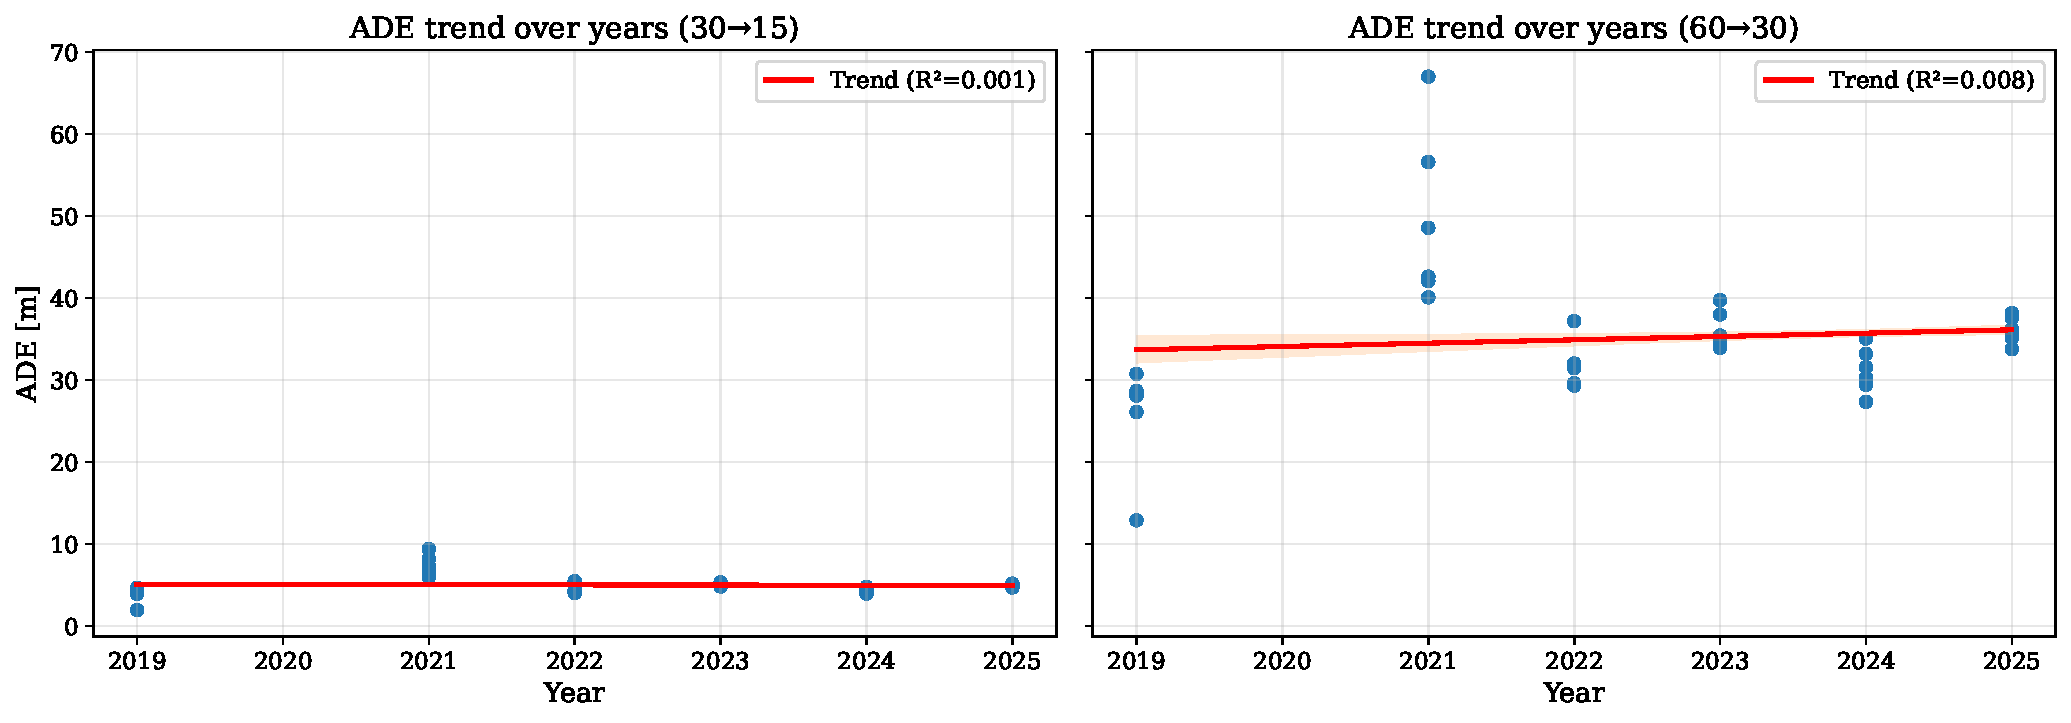
\includegraphics[width=0.95\linewidth]{results/2.ADExYear_en.pdf}
    \caption{Evolution of the seq2seq ADE over the years, separated by prediction horizon.}
    \label{fig:ade_por_ano}
\end{figure}

This result is consistent with the \textit{data drift} hypothesis: the model was trained on a distribution associated with 2019 and loses performance when applied to later seasons. The separation by horizon also shows that the deterioration is not necessarily identical between shorter and longer prediction tasks, reinforcing the usefulness of analyzing the two scenarios independently.

The reading of these plots should be mostly descriptive. The goal here is to establish the basic fact that there is temporal degradation of the absolute error of the model, not yet to explain its mechanism.

\subsection{Comparison with Kalman Filter}

Figure~\ref{fig:seq_kalman} compares the ADE of the seq2seq with that of the Kalman filter over the years, again separating the prediction horizons. The central result is that the seq2seq remains better than the Kalman filter, but the gap between the two grows in the most recent seasons.

\begin{figure}
    \centering
    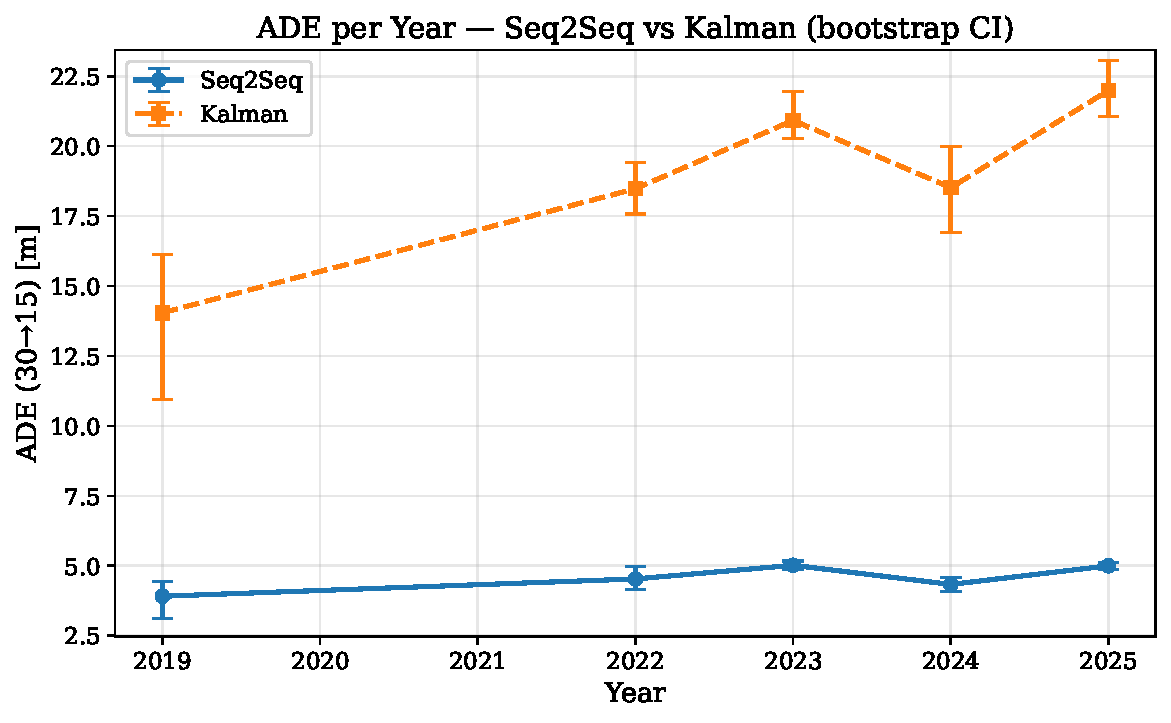
\includegraphics[width=0.95\linewidth]{results/3.Seq2seqVsKalman_en.pdf}
    \caption{Comparison of ADE between Seq2Seq and Kalman over the years, separated by horizon.}
    \label{fig:seq_kalman}
\end{figure}

This evidence must be interpreted carefully. The growing relative advantage of the seq2seq does not mean it is stable. The previous subsection already showed that the absolute error of the seq2seq itself also grows. The correct conclusion is that both methods suffer temporal degradation, but the Kalman filter appears more sensitive to the change of distribution.

Figure~\ref{fig:perc_ade} reinforces this interpretation by showing the percentage increase of the ADE of each method with respect to 2019, for each horizon. In virtually every analyzed year, the percentage growth of the Kalman filter error exceeds that of the seq2seq.

\begin{figure}
    \centering
    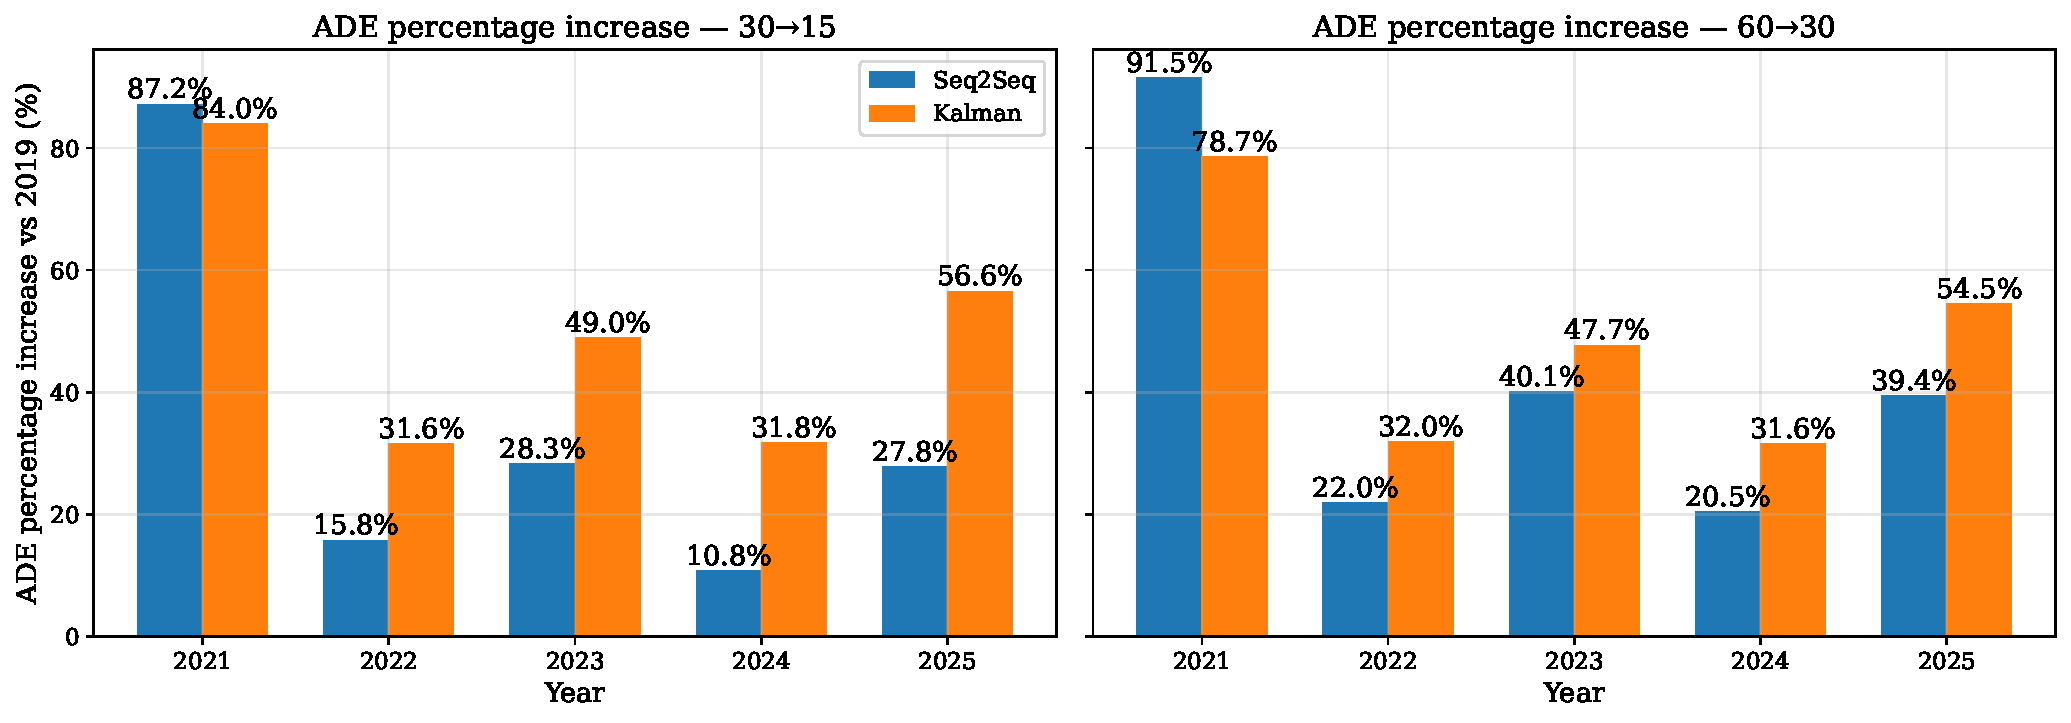
\includegraphics[width=0.95\linewidth]{results/1.PercADE_en.pdf}
    \caption{Percentage increase of ADE with respect to 2019 for Seq2Seq and Kalman, separated by horizon.}
    \label{fig:perc_ade}
\end{figure}

This point matters because it shifts the reading of the paper. The main result is not simply that the seq2seq beats the Kalman filter, but that it appears to degrade less as the game dynamics moves away from the training distribution. In practical terms, this suggests greater relative robustness of the neural model, without eliminating the drift problem.

\subsection{Drift in Kinematic Variables}

To investigate possible mechanisms behind the performance deterioration, we measure distributional drift in the kinematic variables (speed, acceleration, and turn rate) computed from the match data of each season relative to the 2019 baseline. Two families of nonparametric measures are used. The Kolmogorov--Smirnov (KS) statistic~\cite{kolmogorov} quantifies the maximum absolute difference between two empirical cumulative distribution functions; a value close to zero means the distributions are nearly identical, while a value close to one signals a large shift. The Wasserstein distance~\cite{villani} (also known as the earth-mover's distance) measures the minimum transport cost to reshape one distribution into another; larger values indicate greater divergence. Both measures are computed per variable and per year.

Figure~\ref{fig:ks_wd} shows the yearly evolution of the KS and WD metrics for each kinematic variable. The reader should focus on the trend over years: a persistent increase in these metrics from 2019 onwards indicates that the kinematic distributions are progressively moving away from the training-year baseline. Values that fluctuate around zero would, conversely, suggest distributional stability.

\begin{figure}
    \centering
    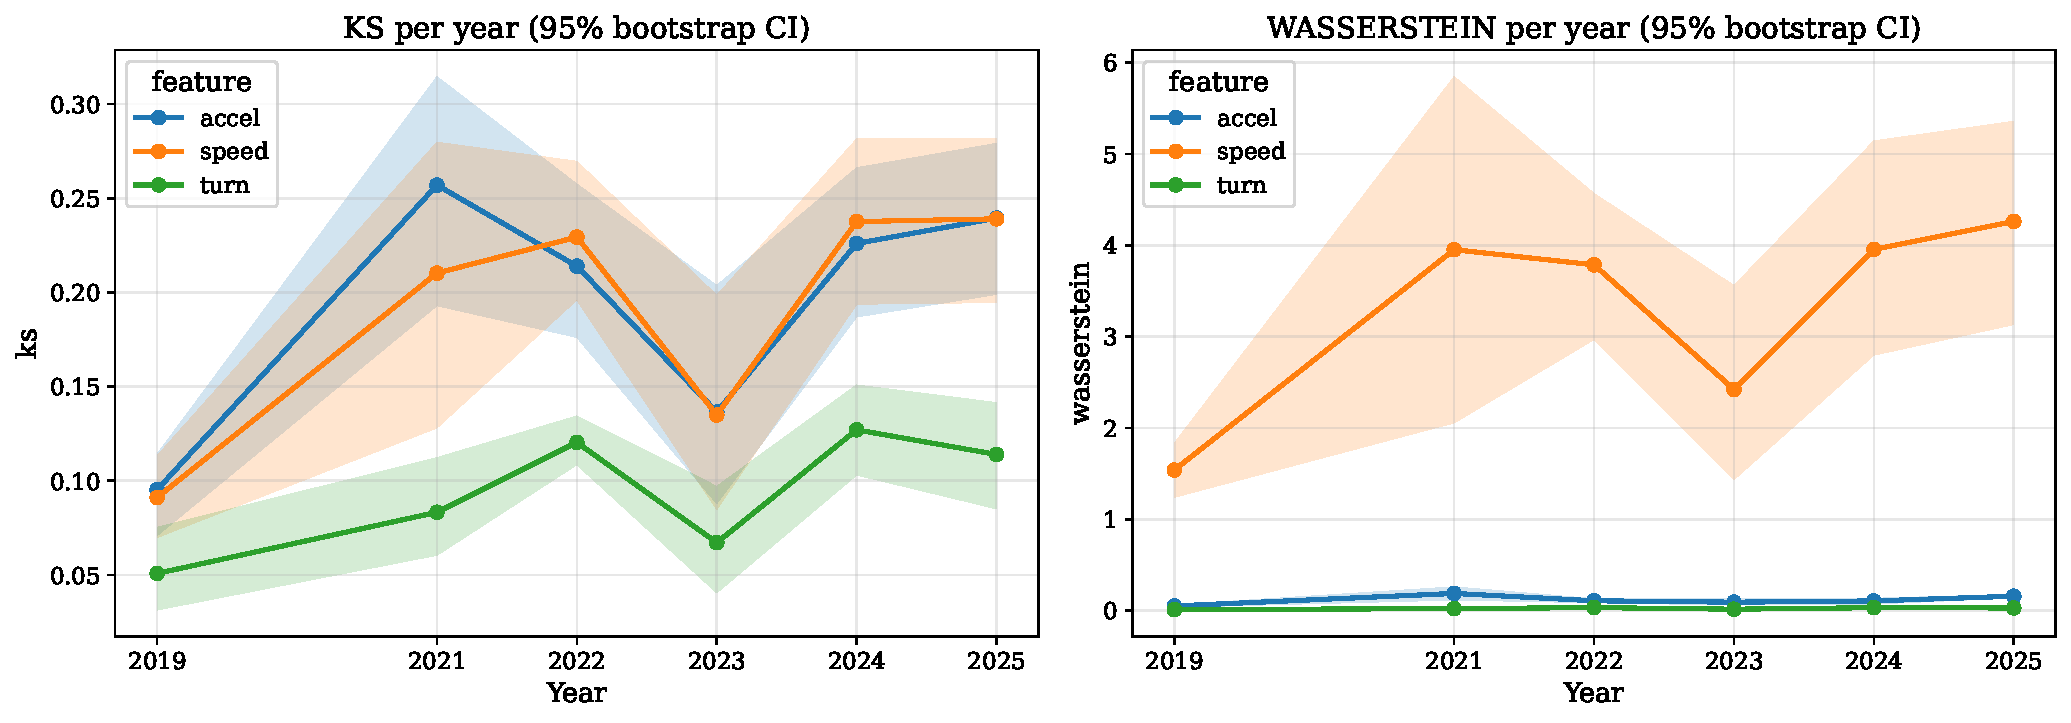
\includegraphics[width=0.95\linewidth]{results/5.KS_WD_xYear_en.pdf}
    \caption{Yearly evolution of KS and WD drift metrics for speed, acceleration, and turn-rate variables, computed relative to the 2019 baseline. Rising values indicate increasing distributional shift away from the training distribution.}
    \label{fig:ks_wd}
\end{figure}

These plots do not prove that the drift in kinematic variables causes the ADE increase. Still, they are informative because they show that performance degradation happens together with measurable changes in the distributions of the variables that describe the game dynamics.

In particular, speed and acceleration display clearer signs of distributional change in later years. This is consistent with the hypothesis that SSL matches became faster, with more aggressive transitions and motions less aligned with the simplifying assumptions of the constant-velocity kinematic model. The turn-rate variable is also relevant, but the signal is less dominant than for speed and acceleration.

\subsection{OLS Regression Analysis}

As a complement to the descriptive analysis, we fit the following models:

\begin{equation}\label{eq:ols_ks}
\Delta ADE \sim ks\_speed + ks\_accel + ks\_turn + C(year),
\end{equation}
\begin{equation}\label{eq:ols_wd}
\Delta ADE \sim wd\_speed + wd\_accel + wd\_turn + C(year).
\end{equation}

Here, \(\Delta ADE\) denotes the variation of the ADE with respect to the 2019 base year, while \(C(year)\) introduces year fixed effects. The role of this regression is neither to identify causality nor to definitively decompose the source of the error. Its function in this paper is more modest: to check whether observable drift metrics maintain association with the variation of ADE after controlling for mean differences across years.

Figure~\ref{fig:ols_ks_wd} shows the estimated coefficients and their confidence intervals for each drift \textit{feature}, separately for the two horizons and for the two families of metrics (KS and WD), allowing us to identify which drift variables keep significant association with \(\Delta ADE\) after the year control.

\begin{figure}
    \centering
    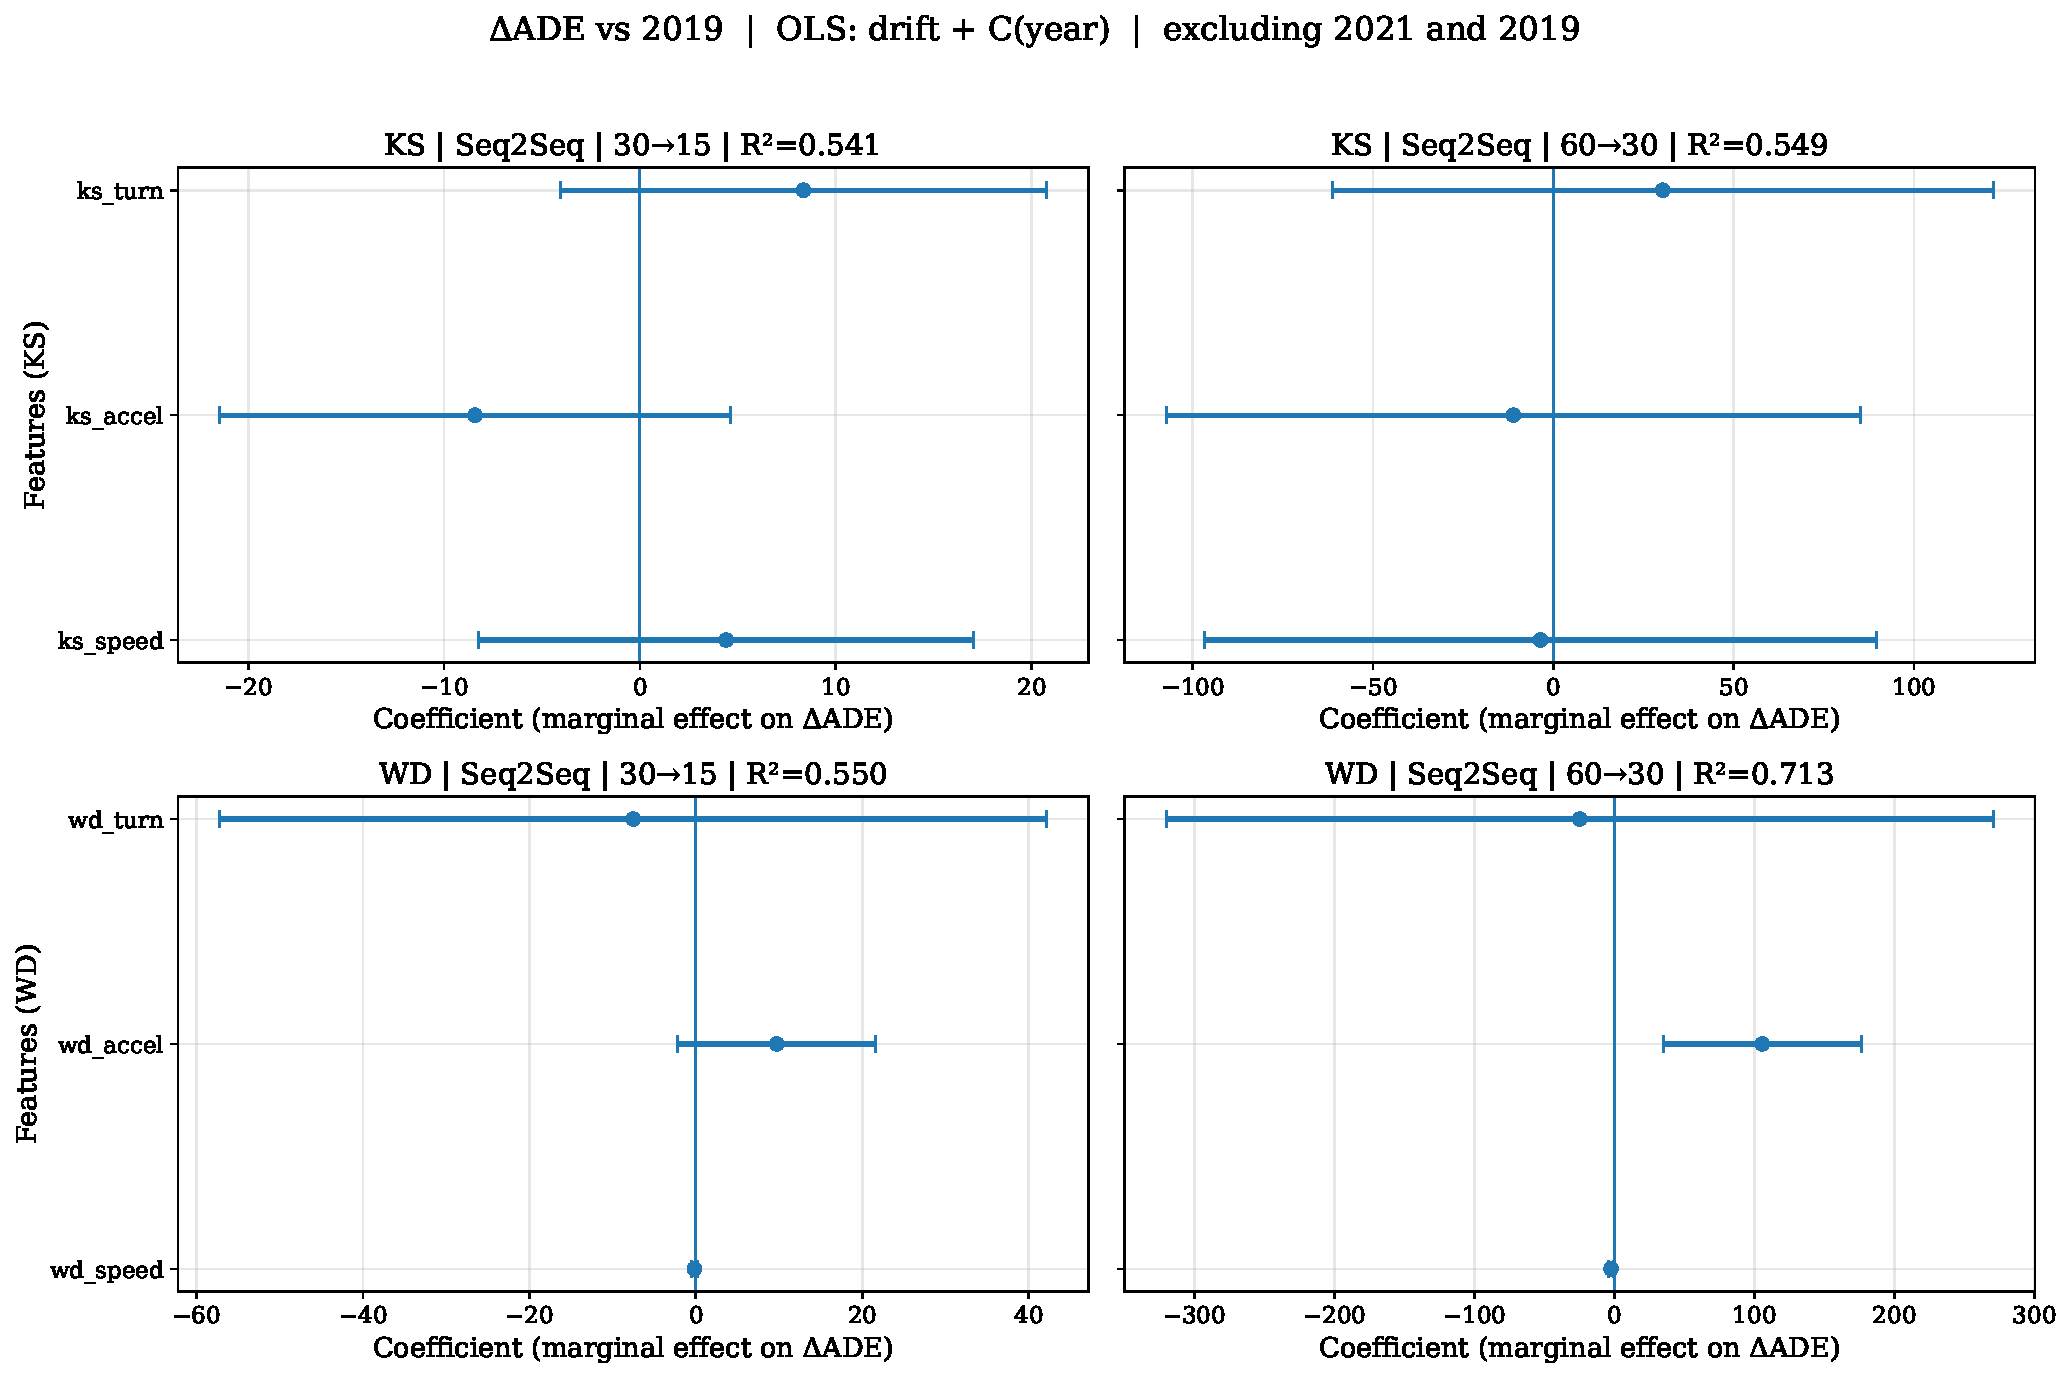
\includegraphics[width=0.9\linewidth]{results/6.OLS_KS_WD_en.pdf}
    \caption{Visual summary of the OLS analysis relating \(\Delta ADE\) with drift metrics.}
    \label{fig:ols_ks_wd}
\end{figure}

The interpretation of this section requires caution for at least three reasons. First, the analysis works with low temporal granularity, which limits inferential power. Second, drift and year share a strong temporal structure, so part of the variation carried by the KS and WD metrics is also captured by the yearly fixed effects. Third, the drift metrics themselves may be correlated, especially when they describe similar changes in the kinematic distributions.

Despite these limitations, the OLS is still useful as an exploratory exercise. Positive coefficients for \(ks\_speed\), \(ks\_accel\), \(ks\_turn\) or their WD counterparts indicate that greater drift in these variables tends to come together with a larger error increase. Thus, the regression does not close the issue, but reinforces the qualitative reading of the earlier plots: the ADE deterioration does not appear to be purely random, but rather associated with observable changes in the game dynamics.

In other words, this section should be read as a starting point for a stronger inference agenda, not as its final step.

Across all analyses, three main messages emerge. First, the seq2seq model suffers temporal performance degradation: the increase of ADE in seasons after training is consistent with the presence of \textit{data drift}. Second, the relative advantage of the seq2seq over the Kalman filter grows over time, suggesting that the classical kinematic benchmark is even more sensitive to SSL regime changes---greater relative robustness does not imply absence of drift, only less pronounced deterioration. Third, part of that error variation appears to track observable drift measures in the kinematic variables; this is supported by the KS and WD series together with the OLS analysis, but should still be understood as suggestive rather than conclusive evidence.

The main contribution of the work is empirical and diagnostic: to show that performance outside the training period deteriorates and that this deterioration is consistent with a change in distribution. The econometric part enters as analytical support, helping to organize hypotheses about the drift mechanism, but not yet resolving them causally. The advance relative to Steuernagel and M\'aximo~\cite{seq2seq} lies in shifting the research question: instead of only asking whether the seq2seq beats the benchmark on a fixed data slice, we ask how that gain evolves as the temporal distribution of the data moves away from the training environment.

\section{Conclusions and Future Work}

We analyzed the temporal stability of a seq2seq model for trajectory prediction in the RoboCup SSL. Results show that the model loses performance in seasons after training, characterizing data drift. They also show that the relative error increase of the Kalman filter predictor is larger, which widens the comparative advantage of the seq2seq in more recent seasons.

The main conclusion is twofold. First, there is clear evidence of temporal degradation in the seq2seq. Second, the Kalman filter predictor appears to be even more affected by the temporal shift of the data distribution. The KS and WD metrics, together with the OLS analysis, reinforce the interpretation that the error increase tracks measurable changes in the observed dynamics of the matches.

The OLS regression should be read as complementary exploratory analysis, useful for guiding hypotheses and next tests, but insufficient to support causality. This work extends the line opened by Steuernagel and M\'aximo~\cite{seq2seq} from the problem of pointwise performance to the problem of temporal stability.

This study has important limitations. The analysis is anchored to a single training year (2019), making it impossible to isolate the effect of that specific training dataset from a general temporal trend. The yearly granularity produces few data points for the OLS analysis, limiting statistical power and the ability to distinguish the individual contribution of each drift feature. The exclusion of 2020 and 2021 due to a structural rupture in the competition creates gaps in the temporal series. Furthermore, both the seq2seq model and the Kalman filter predictor were parameterized from 2019 data, so neither serves as a fully distribution-free baseline against which to measure drift.

Regarding future work, a natural next step is to move from aggregated yearly analysis to a more granular base---per match, time window, or play block---to observe intra-year variation and better separate the effect of time from the effect of measured drift. An interesting extension is to use as dependent variable the difference \(ADE^{\mathrm{Kalman}} - ADE^{\mathrm{Seq2Seq}}\) or its relative ratio, studying in which contexts drift further amplifies the comparative advantage of the neural model. Periodic model retraining and domain adaptation strategies~\cite{gama2014} could also be investigated as practical countermeasures to the observed degradation.

\section*{Acknowledgements}
Ivan Yamasaki acknowledges the support of ITAEx and Nubank, provided within the framework of the ITA Undergraduate Research Program in Artificial Intelligence (2025--2026).

\begin{thebibliography}{9}

\bibitem{sutskever}
Sutskever, I., Vinyals, O., Le, Q. V.: Sequence to Sequence Learning with Neural Networks. In: Advances in Neural Information Processing Systems, vol. 27 (2014)

\bibitem{seq2seq}
Steuernagel, L., M\'aximo, M. R. O. A.: Trajectory Prediction for SSL Robots Using Seq2seq Neural Networks. In: Eguchi, A., Lau, N., Paetzel-Pr\"usmann, M., Wanichanon, T. (eds.) RoboCup 2022: Robot World Cup XXV. LNCS, vol. 13561, pp. 27--38. Springer, Cham (2023). doi:10.1007/978-3-031-28469-4\_4

\bibitem{bahdanau}
Bahdanau, D., Cho, K., Bengio, Y.: Neural Machine Translation by Jointly Learning to Align and Translate. In: 3rd International Conference on Learning Representations (ICLR) (2015)

\bibitem{kalman}
Kalman, R. E.: A New Approach to Linear Filtering and Prediction Problems. Journal of Basic Engineering \textbf{82}(1), 35--45 (1960)

\bibitem{adam}
Kingma, D. P., Ba, J.: Adam: A Method for Stochastic Optimization. In: 3rd International Conference on Learning Representations (ICLR) (2015)

\bibitem{barrat}
Barratt, S. T., Boyd, S. P.: Fitting a Kalman Smoother to Data. In: 2020 American Control Conference (ACC), pp. 1526--1531 (2020). doi:10.23919/ACC45564.2020.9147485

\bibitem{kolmogorov}
Kolmogorov, A. N.: Sulla determinazione empirica di una legge di distribuzione. Giornale dell'Istituto Italiano degli Attuari \textbf{4}, 83--91 (1933)

\bibitem{villani}
Villani, C.: Optimal Transport: Old and New. Grundlehren der mathematischen Wissenschaften, vol. 338. Springer, Berlin (2009)

\bibitem{kitano1997}
Kitano, H., Asada, M., Kuniyoshi, Y., Noda, I., Osawa, E.: RoboCup: The Robot World Cup Initiative. In: Proceedings of the First International Conference on Autonomous Agents, pp. 340--347. ACM Press (1997)

\bibitem{alahi2016}
Alahi, A., Goel, K., Ramanathan, V., Robicquet, A., Fei-Fei, L., Savarese, S.: Social LSTM: Human Trajectory Prediction in Crowded Spaces. In: IEEE Conference on Computer Vision and Pattern Recognition (CVPR), pp. 961--971 (2016)

\bibitem{salzmann2020}
Salzmann, T., Ivanovic, B., Chakravarty, P., Pavone, M.: Trajectron++: Dynamically-Feasible Trajectory Forecasting with Heterogeneous Data. In: Vedaldi, A. et al. (eds.) ECCV 2020, LNCS, vol. 12363, pp. 683--700. Springer (2020)

\bibitem{gama2014}
Gama, J., \v{Z}liobait\.e, I., Bifet, A., Pechenizkiy, M., Bouchachia, A.: A Survey on Concept Drift Adaptation. ACM Computing Surveys \textbf{46}(4), 1--37 (2014)

\bibitem{yan2014}
Yan, S., Cao, X.: Applied Research to Predict the Position of the Robot Soccer Game and the Kalman Filter Algorithm. BioTechnology: An Indian Journal \textbf{10}(10), 4634--4642 (2014)

\bibitem{yuan2015}
Yuan, C., Li, S.: Implement Prediction of Ball Position in Robot Soccer Using Kalman Filter. In: 2015 6th International Conference on Manufacturing Science and Engineering (ICMSE). Atlantis Press (2015)

\bibitem{ryang2016}
Ryang, G., Choe, M., Sin, Y.: Position Prediction of Ball and Fuzzy Controller for Shooting Action in a Soccer Robot System. arXiv preprint arXiv:1604.05790 (2016)

\end{thebibliography}

\end{document}
